\documentclass{article}
\usepackage[utf8]{inputenc}
\usepackage{geometry}

 \geometry{
 a4paper,
 total={170mm,257mm},
 left=20mm,
 top=20mm,
 }
 
\title{Project 3 – Nature-Inspired Algorithms}
\author{Lawrence Benson, Willi Gierke, Nico Ring}
\date{$10^{\textnormal{\small{th}}}$ July 2017}

\usepackage{natbib}
\usepackage{graphicx}

\usepackage{amsfonts,amsmath,amssymb}
\usepackage{amsthm}
\usepackage{graphicx}
\usepackage{xcolor}
%\usepackage{ngerman}
\usepackage{listings}
\usepackage[utf8]{inputenc}
%\usepackage[T1]{fontenc}
\usepackage{comment}
\usepackage{algorithm}
\usepackage{hyperref}
%%\usepackage{algpseudocode} 
\renewcommand*\thealgorithm{}
\usepackage{algorithmic}

\newtheorem{theorem}{Theorem}



\begin{document}

\maketitle

\section{Algorithm Modifications}
Most of our algorithm is based on the description given in the task. We adapted the algorithm a bit as described in \href{https://svn-d1.mpi-inf.mpg.de/AG1/MultiCoreLab/papers/StuetzleHoos00\%20-\%20MMAS.pdf}{\textit{Stützle and Hoos paper}}. We changed the following things:
\begin{itemize}
    \item{Init all pheromones with $\tau_{max}$ instead of $\tau_{min}$. This allows for a larger exploration of the problem space at the beginning.}
    \item{We don't use 1 ant per iteration, but 5. This gives a small speed up, because updating the pheromones is an expensive operation.}
    \item{Furthermore, we don't always lay the pheromones according to the global best tour (so far), but also use the best tour from an iteration. This allows us to explore more paths instead of running into a local minimum and not getting out again, as the pheromones are to strong.}
    \item{If we have not improved for 5000 iterations, we reset the pheromones to get out of the local minimum.}
    \item{After 3000 iterations without improvement, we increase the pheromones on all edges for the same reason as initializing all edges with $\tau_{max}$.}
\end{itemize}
\section{Evaluation}

\subsection{Effect of $\alpha$ and $\beta$}
We evaluated the effect on the convergence to the optimum of the weights $\alpha$ and $\beta$ for the pheromones and edge weights respectively. Therefor, we run the algorithm on the \textit{gr202} dataset with different values for both parameters and measured the deviation to the optimum after 5000 iterations. We did this five times for each pair of parameters and took the average of the resulting deviations.
\begin{figure}[h]
  \center
  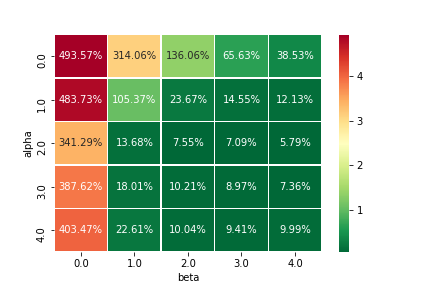
\includegraphics[width=0.5\paperwidth]{alpha-beta-heatmap.png}
  \caption{Devation values for different $\alpha$ and $\beta$ values after 5000 iterations.}
  \label{fig:alpha-beta}
\end{figure}
\\
Figure~\ref{fig:alpha-beta} shows the results of testing the effect of $\alpha$ and $\beta$ on the convergence to the optimum. First of all, we see that if one of both values is zero, thus having no effect on the probability to choose an edge, the deviation values are much higher compared to the other values. Only for values $\beta \geq 3$ we get a reasonable deviation from the optimum. So only using the edge weight heuristic can produce reasonable results, but only using the pheromone heuristic not. For parameter pairs with $\alpha \neq 0$ and $\beta \neq 0$, $\alpha = 2$ seems to be a good choice for this data set, because for smaller and larger values we get worse results. Furthermore, for this dataset the following holds: the larger beta the better are the results we get. All in all, we conclude that you can achieve the best results if you combine the pheromone and edge weight heuristics.


\subsection{Runtime}

\begin{figure}[h]
  \center
  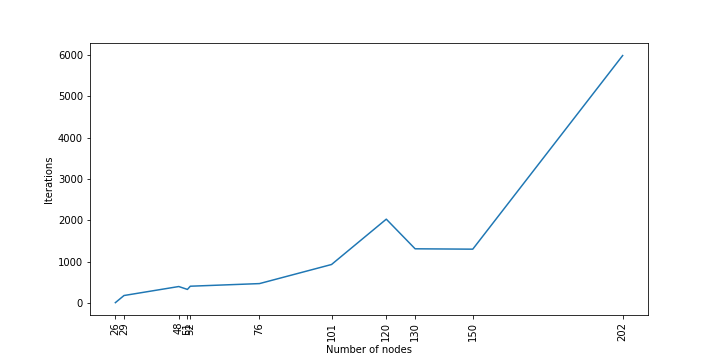
\includegraphics[width=0.7\paperwidth]{Goal_10.png}
  \caption{Iterations needed to achieve a deviation of at most 10\% from the optimum for different instances.}
  \label{fig:goal10}
\end{figure}

\begin{figure}[h]
  \center
  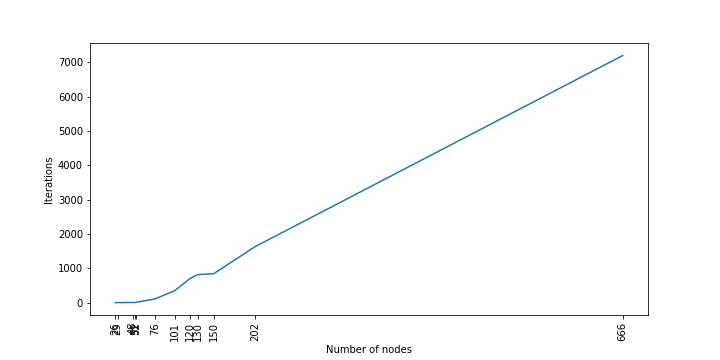
\includegraphics[width=0.7\paperwidth]{Goal_30.png}
  \caption{Iterations needed to achieve a deviation of at most 30\% from the optimum for different instances.}
  \label{fig:goal30}
\end{figure}

\begin{figure}[h]
  \center
  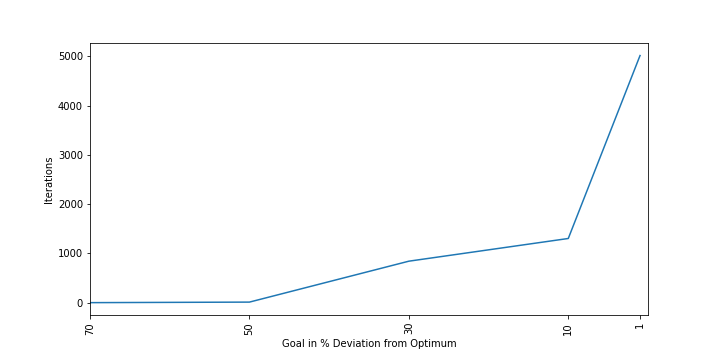
\includegraphics[width=0.7\paperwidth]{Nodes_150.png}
  \caption{Iterations needed on an instance with 150 cities to achieve different deviations from the optimal solution.}
  \label{fig:nodes150}
\end{figure}

\begin{figure}[h]
  \center
  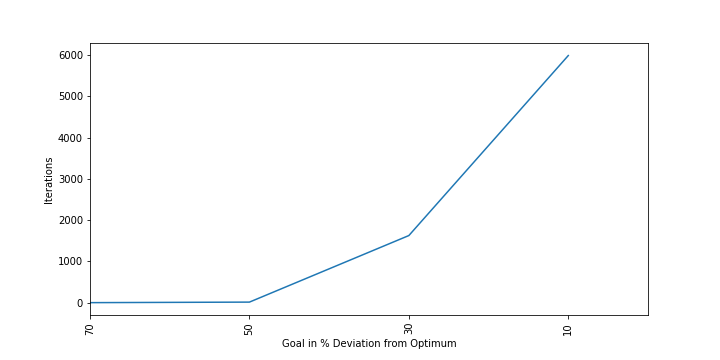
\includegraphics[width=0.7\paperwidth]{Nodes_202.png}
  \caption{Iterations needed on an instance with 202 cities to achieve different deviations from the optimal solution.}
  \label{fig:nodes202}
\end{figure}
\\
In Figure \ref{fig:goal30} we can see that the number of iterations to reach a deviation of 10\% from the optimal solution nearly grows linearly in the number of involved nodes. Figure \ref{fig:goal10} disproves the theory that this might be the general behavior, independent from the number of nodes. Instead, Figure \ref{fig:goal10} shows that the number of iterations grows exponentially with respect to the number of involved cities. This creates the theory that the number of needed iterations might be heavily dependent on the desired maximum deviation.\\
Figures \ref{fig:nodes150} and \ref{fig:nodes202} undergrid this thesis.
As we can clearly tell from them, the number of iterations grows exponentially with respect to the desired maximum deviation from the optimal solution regarding different instances.

\section{Bonus Tasks}

Our setup for the following tasks included a MacBook Pro running a 2 GHz Intel Core i7 processor with 8 GB 1600 MHz DDR3 main memory. For bigger instances we used a server hosted by the FSOC lab powering 40 2 Ghz cores and 128 GB RAM. Every task ran on one core with one thread.

\subsection{$40+$ cities optimally}
We solved the instance \textit{berlin52} with 52 cities optimally in 4659 iterations. The tour can be found in berlin52.res in the zip file.

\subsection{$100+$ cities at 1\%}
We solved \textit{ch130} with 130 cities within $1\%$ in 6067 iterations. The tour can be found in ch130.res in the zip file.\\
We solved \textit{ch150} with 150 cities within $1\%$ in 5825 iterations. The tour can be found in ch150.res in the zip file.
It took approximately 2 hours to compute the solutions.

\subsection{$1000+$ cities at 30\%}
no :(


\subsection{Largest instance at 50\%}
We solved \textit{pla7397} with 7397 cities within $50\%$. We solved this 3 times within the first iteration. We observed that this instance seems to be easy to solve in general. We observed that it can be solved with heuristic information alone, i.e. we set $\alpha = 0$, so no pheromones were used and also managed to solve this instance in a few iterations. The tour can be found in pla7397.res in the zip file.
It took us approximately 5 hours to compute the solution.
\end{document}